\chapter{Background}
%labels will help you to reference to certain images, tables, chapters, section, and so on...
\label{background}



%DELETEME: This chapter will cover all of your background information and related work. Background and related work are directly related to your thesis. Please do not place irrelevant content here which is a common mistake. Citing will be handled in the appendices.

In this chapter we discuss Amazon's state-of-the-art strategy before moving on to related work in other archetypes as it is important to introduce the implementation scope of voice assistants bottom-up prior to exploring the current context within the same boundaries of voice assistants then compare it to other approaches in the larger context of conversational bots as a whole from a technical and user experience point of view. We start juxtaposition of Voice User Interface (VUI) to the Graphical User interface (GUI) with respect to cognition and behavioural design which gets us to define new terminological foundation that will follow throughout this thesis to then bring implementation requirements to the table in section \ref{frameworks_structs}. 


%DELETEME: Background represents underlying knowledge that is required to understand your work. The expected knowledge level of your readers can be set to the one of a bachelor or master student who just finished his studies (depending on what kind of thesis you are writing). This means that you do not need to describe how computers work, unless your thesis topic is about this. Everything that an avarage alumni from your field of studies should know does not need to be described. It turn, background information that is very complex and content-wise very near to you problem, can be placed in the main parts. Everyting else should be written here. Note: it is important to connect each presented topic to your thesis. E.g. if you present the ISO/OSI layer model you should also write that this is needed to understand the protocols you plan to develop in the main parts.

\subsection*{VUI vs. GUI} 

etkallem 3an el paradigm shift eli 7asal ma3 el mouse from cli if not already mentioned
then 3an el smartphones and the wep from wap etc (deskop version, responsive design, two versions, em instead of pt, relative, starting with a tablet and a phone then anything relative to those then when the standards showed that there won't be an only 15 inch and a 12 inch there will be everything in between, we changed the idea to include continuous units in the spectrum and not only discrete units)
\cite{alexa_19}
different screens, different mobile experiences and what does it mean

how do you think of designing voice when you have a mobile mindset
how do you think about screens when you have a mobile mindset and thinking about voice
subtle differnce



\subsection{VUI Terminology} \todo{explain json}
\begin{itemize}
	\item[intent]
	\item[utterance]
	\item [slot]
\end{itemize}


gui in vui *card display* alexa podcast el adima that i heard while running i think


imagine you have an intent and the label on th button says ok

%#################################################################################
%###################### State of the Art  ########################################
%#################################################################################
\section{State of the Art}


\subsection*{Amazon Web Services (AWS) + Alexa}


Getting started with Alexa as a platform for the first time might seem a little overwhelming especially since each component of it is being  constantly restructured since its debut release in November 2014 and with Q4 2016 being the beginning of its major market penetration success \cite{gartnerpreds17}. % AWS is constantly working on the interface and the sdk 
As throughout the course of this thesis these major changes occurred, %including even logo changes of the AWS modules!
%do some kind of changelog later
 we will go over the workarounds and circumventions to retain a working version of the software we present, discuss


\subsubsection*{AWS}
Amazon Web Services is a Cloud Computing service provider with a complete set of services to help build and run web applications ``reliably and securely at a cost and scale'' according to one's independent needs. \cite{aws_website}
It comes with agile abilities to adjust to various solution at a flexible scheme with benefits like multiple server farms globally (operating under different legal contracts with respect to data security and user privacy), caching, NoSQL, DevOps and so forth.


\subsubsection*{Alexa}
Alexa is a cloud-based voice service assistant platform by Amazon powering millions of devices \inote{with {number of requests} {daily|monthly}} on its own-branded devices like the Echo, Echo Dot, Tap, FireTV as well as cross-platform through mobile apps available through  \href{https://itunes.apple.com/de/app/amazon-alexa/id944011620?l=en&mt=8}{Apple's AppStore for iOS} and  \href{https://play.google.com/store/apps/details?id=com.amazon.dee.app&hl=en}{Google Play Store for Android} devices. Unlike Apple's approach with Siri for instance \footnote{as know from its policy on  new software and hardware products like the case with the iPhone, the Mac, etc.}, where including support for third-party integration on iOS's Service Development Kit (SDK), Amazon decided with the launch of Alexa to include non-Amazon developers right from the start by introducing a multitude of (SDKs) around the platform as part of AWS, e.g. Alexa Skills Kit SDK discussed further below.

So far, though the separation of AWS and Alexa's environments is not linguistically intuitive with the company's name labelled on every service component \footnote{see Etymology \ref{etymology}}, \href{http://www.amazon.com}{Amazon.com, Inc.} offers an array of web services through AWS that summarize all building blocks necessary to operate Alexa as a software for end-users. Of course with the introduction of the aforementioned devices, it becomes intuitive to call these `Alexa devices' since their primary purpose is to operate as Alexa clients. We refer to Alexa here only as the service offered by Amazon to consumers. Consequently, although Alexa comes as a fully packaged service to end-users, we can reduce it to a compilation of many micro-services provided by AWS. As most of these are available separately in the form of Software as a Service (Saas), we conclude that AWS incorporates the following components required to make Alexa come together and becomes a consumer of its own web services platform. 

\subsubsection*{Alexa's AWS Modules \inote{make logos as minipage objects or set as table}}
%\inote{in print, make sure the following list goes on a spread (odd then even page number) with the image at the end of it for clarity}

listed in sequential order of importance, Alexa's service modules include but are not limited to: 

\begin{enumerate}

	\item[\href{https://aws.amazon.com/lex/}{\textbf{Lex}} \footnote{\url{https://aws.amazon.com/lex}}] \textit{for conversational interfaces using Natural Language Understanding, Text-to-Speech and Speech-to-Text} \\
	``a service for building conversational interfaces into any application using voice and text''\cite{aws_website}.
	While Lex is the most important backbone to make Alexa possible and can be a main operator of another software package to create a whole new category of voice assistants and conversational bots independent from Alexa, Siri etc., development for Lex was not available in German at the time of this research. We therefore decide to use the Alexa Skills Kit, which take advantage of Lex and the other components described below. Lex and Alexa use the same deep learning techniques for natural language processing with the workflow described with the example in figure \ref{lex_interactionExample}.
	
	\begin{restoretext}
		\begin{flushright}
			%
\includegraphics[width=\linewidth,height=1cm]{template/aot_logo}
			
\includegraphics[width=1cm,height=1.1cm]{awslogos/lexlogo}
		\end{flushright}

	\end{restoretext}

	
	
	\item[\href{https://aws.amazon.com/polly/}{\textbf{Polly}} \footnote{\url{https://aws.amazon.com/polly}}] \textit{for speech synthesis\\}
	another ``service turn[ing] text into lifelike speech, allowing [developers] to create applications that talk'' \cite{aws_website} wile harnessing the power of deep learning. It is more or less the mouthpiece of Alexa built on top of speech synthesis algorithms.
	
	
	\begin{restoretext}
		\begin{flushright}
		
\includegraphics[width=1.06cm,height=0.9cm]{awslogos/pollylogo}
		\end{flushright}
	\end{restoretext}
	
	
	\item[\href{https://aws.amazon.com/transcribe/}{\textbf{Transcribe}} \footnote{\url{https://aws.amazon.com/transcribe}}] \textit{for automatic speech recognition using Speech-to-Text}\\
	which ``makes it easy for developers to add speech-to-text capability to [...] applications'' \cite{aws_website}. With Transcribe we are able to get text out of the user's voice before passing it into a format Alexa's backend would understand.
	
	
	\begin{restoretext}
\begin{flushright}
	
\includegraphics[width=1.2cm,height=0.9cm]{awslogos/transcribelogo}
\end{flushright}
	\end{restoretext}
	
	
	\item[\href{https://aws.amazon.com/lambda/}{\textbf{Lambda}} \footnote{\url{https://aws.amazon.com/lambda}}] \textit{for intent fulfilment}\\
	Although Lambda is a versatile ``service [built] for a variety of real-time serverless data processing systems'' \cite{aws_website}, we use it as an integrated server instance to host our back-end code for intent fulfilment \ref{intent_fulfilment}. We might as well use just any other privately or cloud-based server solution to host our code and use it as an endpoint for our software, however choosing Lambda takes away the overhead of linking the front-end with the back-end of the program we develop (an Alexa Skill as we describe below). 
	
	
	\begin{restoretext}
\begin{flushright}
	
\includegraphics[width=0.8cm,height=0.9cm]{awslogos/lambdalogo}
\end{flushright}
	\end{restoretext}


	\item[\href{https://aws.amazon.com/iam/}{\textbf{CloudWatch}} \footnote{\url{https://aws.amazon.com/cloudwatch}}]
	\textit{for event logging}\\
	CloudWatch acts like the console for an operating system. It monitors all low-level events happening within the AWS sphere. In combination with Lambda it comes as handy tool to log events resulting at runtime once a Lambda instance is called and its code being executed.
	
	
	\begin{restoretext}
\begin{flushright}
	
\includegraphics[width=1.26cm,height=0.9cm]{awslogos/cloudwatchlogo}
\end{flushright}
	\end{restoretext}


	\item[\href{https://aws.amazon.com/iam/}{\textbf{IAM}} \footnote{\url{https://aws.amazon.com/iam}}]
	\textit{for identity access management within AWS}\\
	Identity Access Management (IAM) is a secondary service module regulating in the Alexa context in combination with Lambda the routing rights between internal Amazon endpoints. It also ensures compliance policies are enforced within and between AWS modules, as well as between AWS modules and other external services.
	
	
	\begin{restoretext}
\begin{flushright}
	
\includegraphics[width=1.36cm,height=0.85cm]{awslogos/cognitologo}
\end{flushright}
	\end{restoretext}


	\item[\href{https://aws.amazon.com/cognito/}{\textbf{Cognito}} \footnote{\url{https://aws.amazon.com/cognito}}]
	\textit{for identity access management beyond AWS}\\
	like the rest of AWS's platform, Cognito is a scalable service module to perform user authentication and can be used in combination with an external endpoint instead of Lambda.
	
		\begin{restoretext}
\begin{flushright}
	
\includegraphics[width=0.76cm,height=0.9cm]{awslogos/cognitologo_old}
\end{flushright}
	\end{restoretext}
	
\end{enumerate}

%\newpage

\begin{figure}[h]
	\caption{Interaction between AWS modules in the use case of a ``Coffee Bot'' based on reference \cite{aws:lex_webinar} }\label{lex_interactionExample}
	\centering
	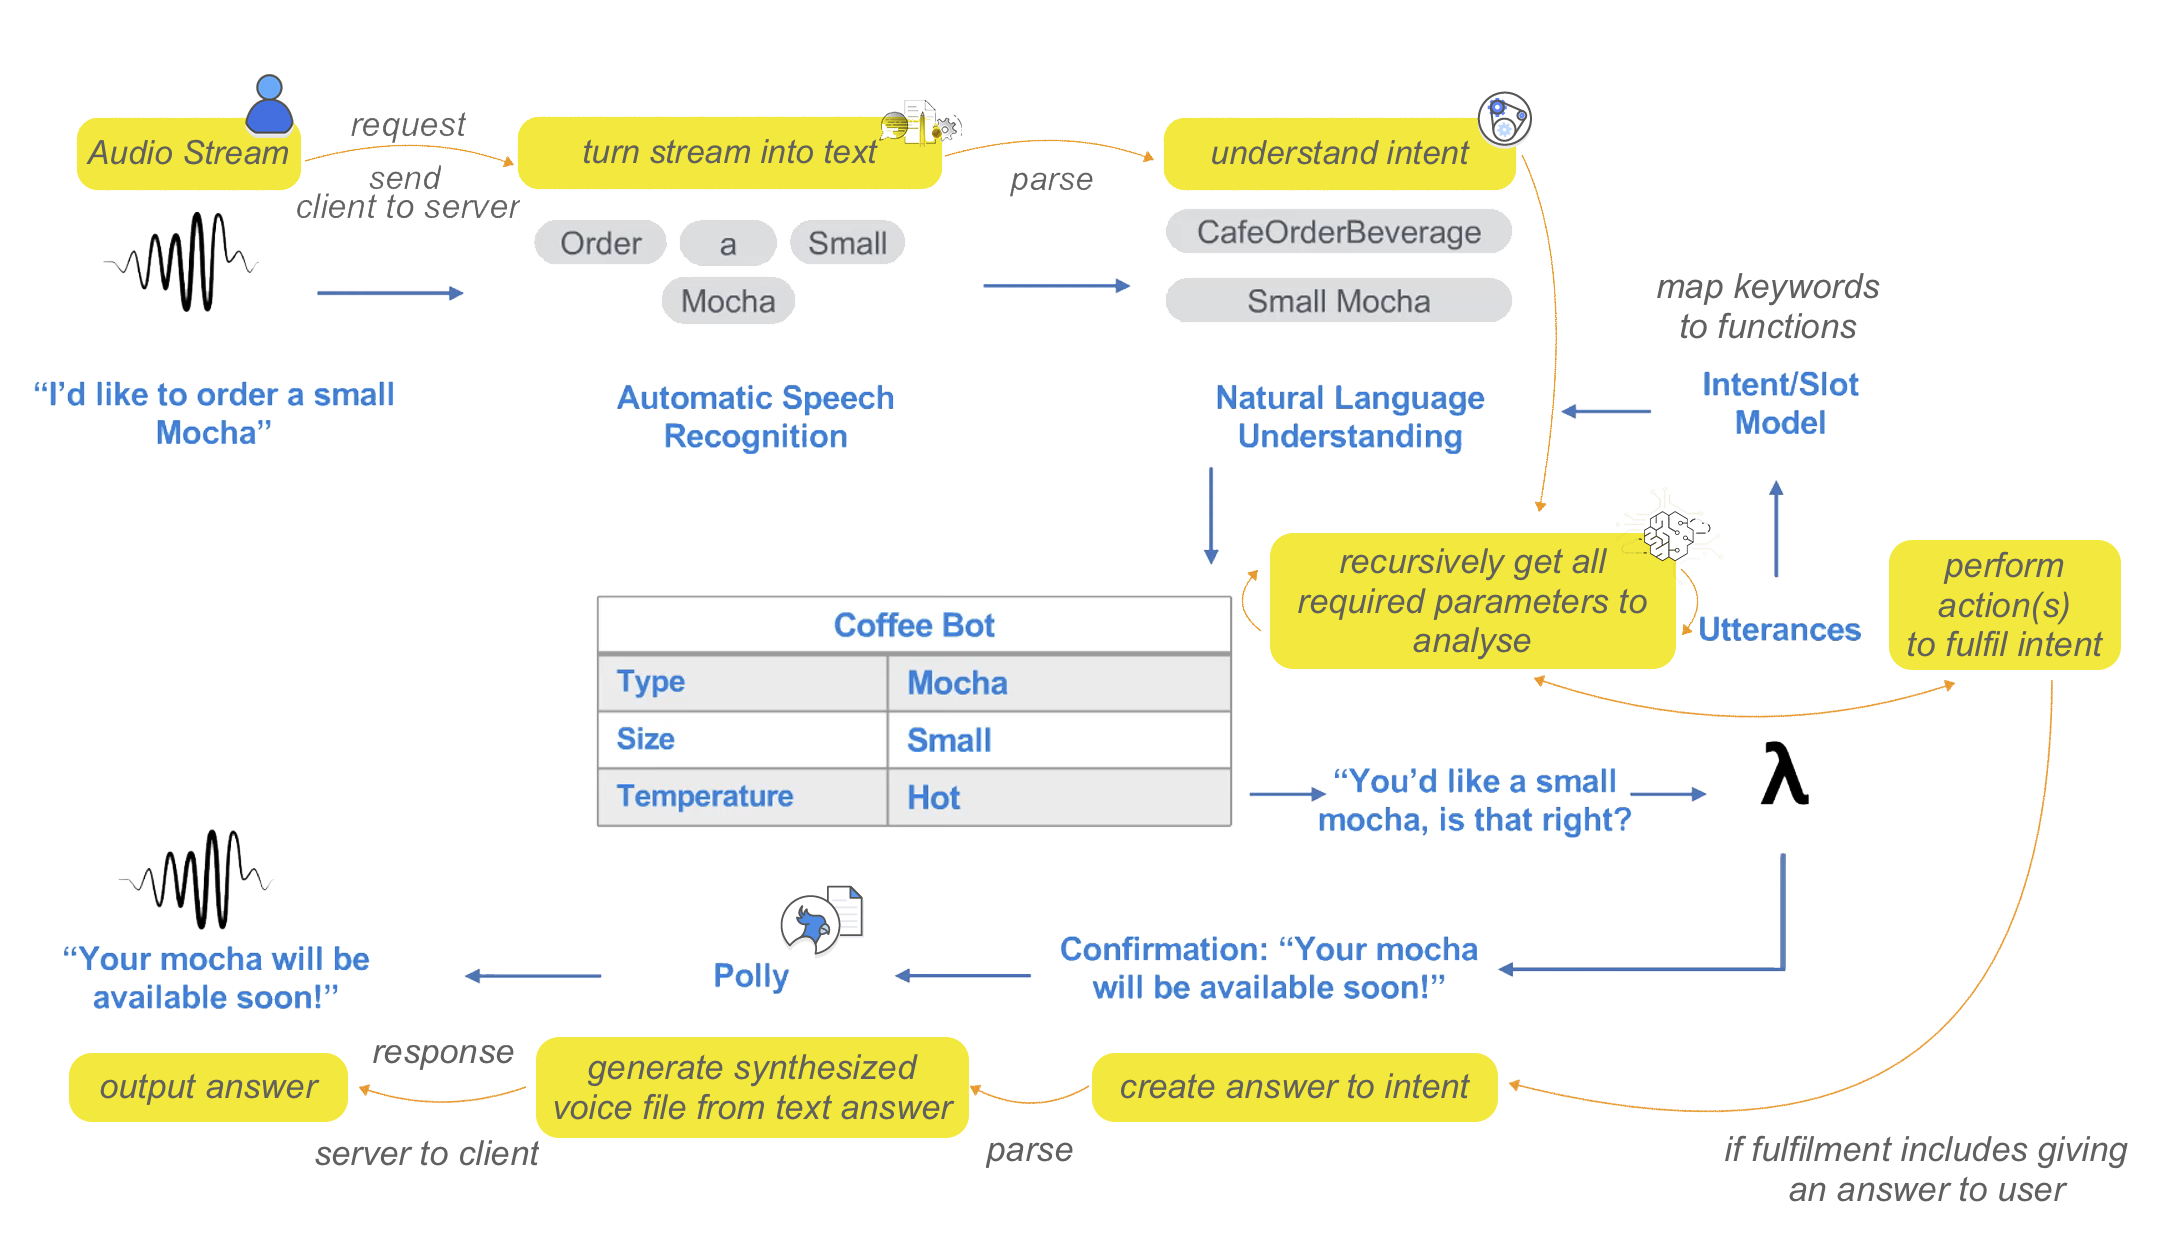
\includegraphics[width=14.8cm]{workflows/awstools.png}
\end{figure}
%
%\begin{wrapfigure}{l}{1.5cm}
%	\caption{Interaction between AWS modules in the use case of a ``Coffee Bot''}\label{lex_interactionExample}
%	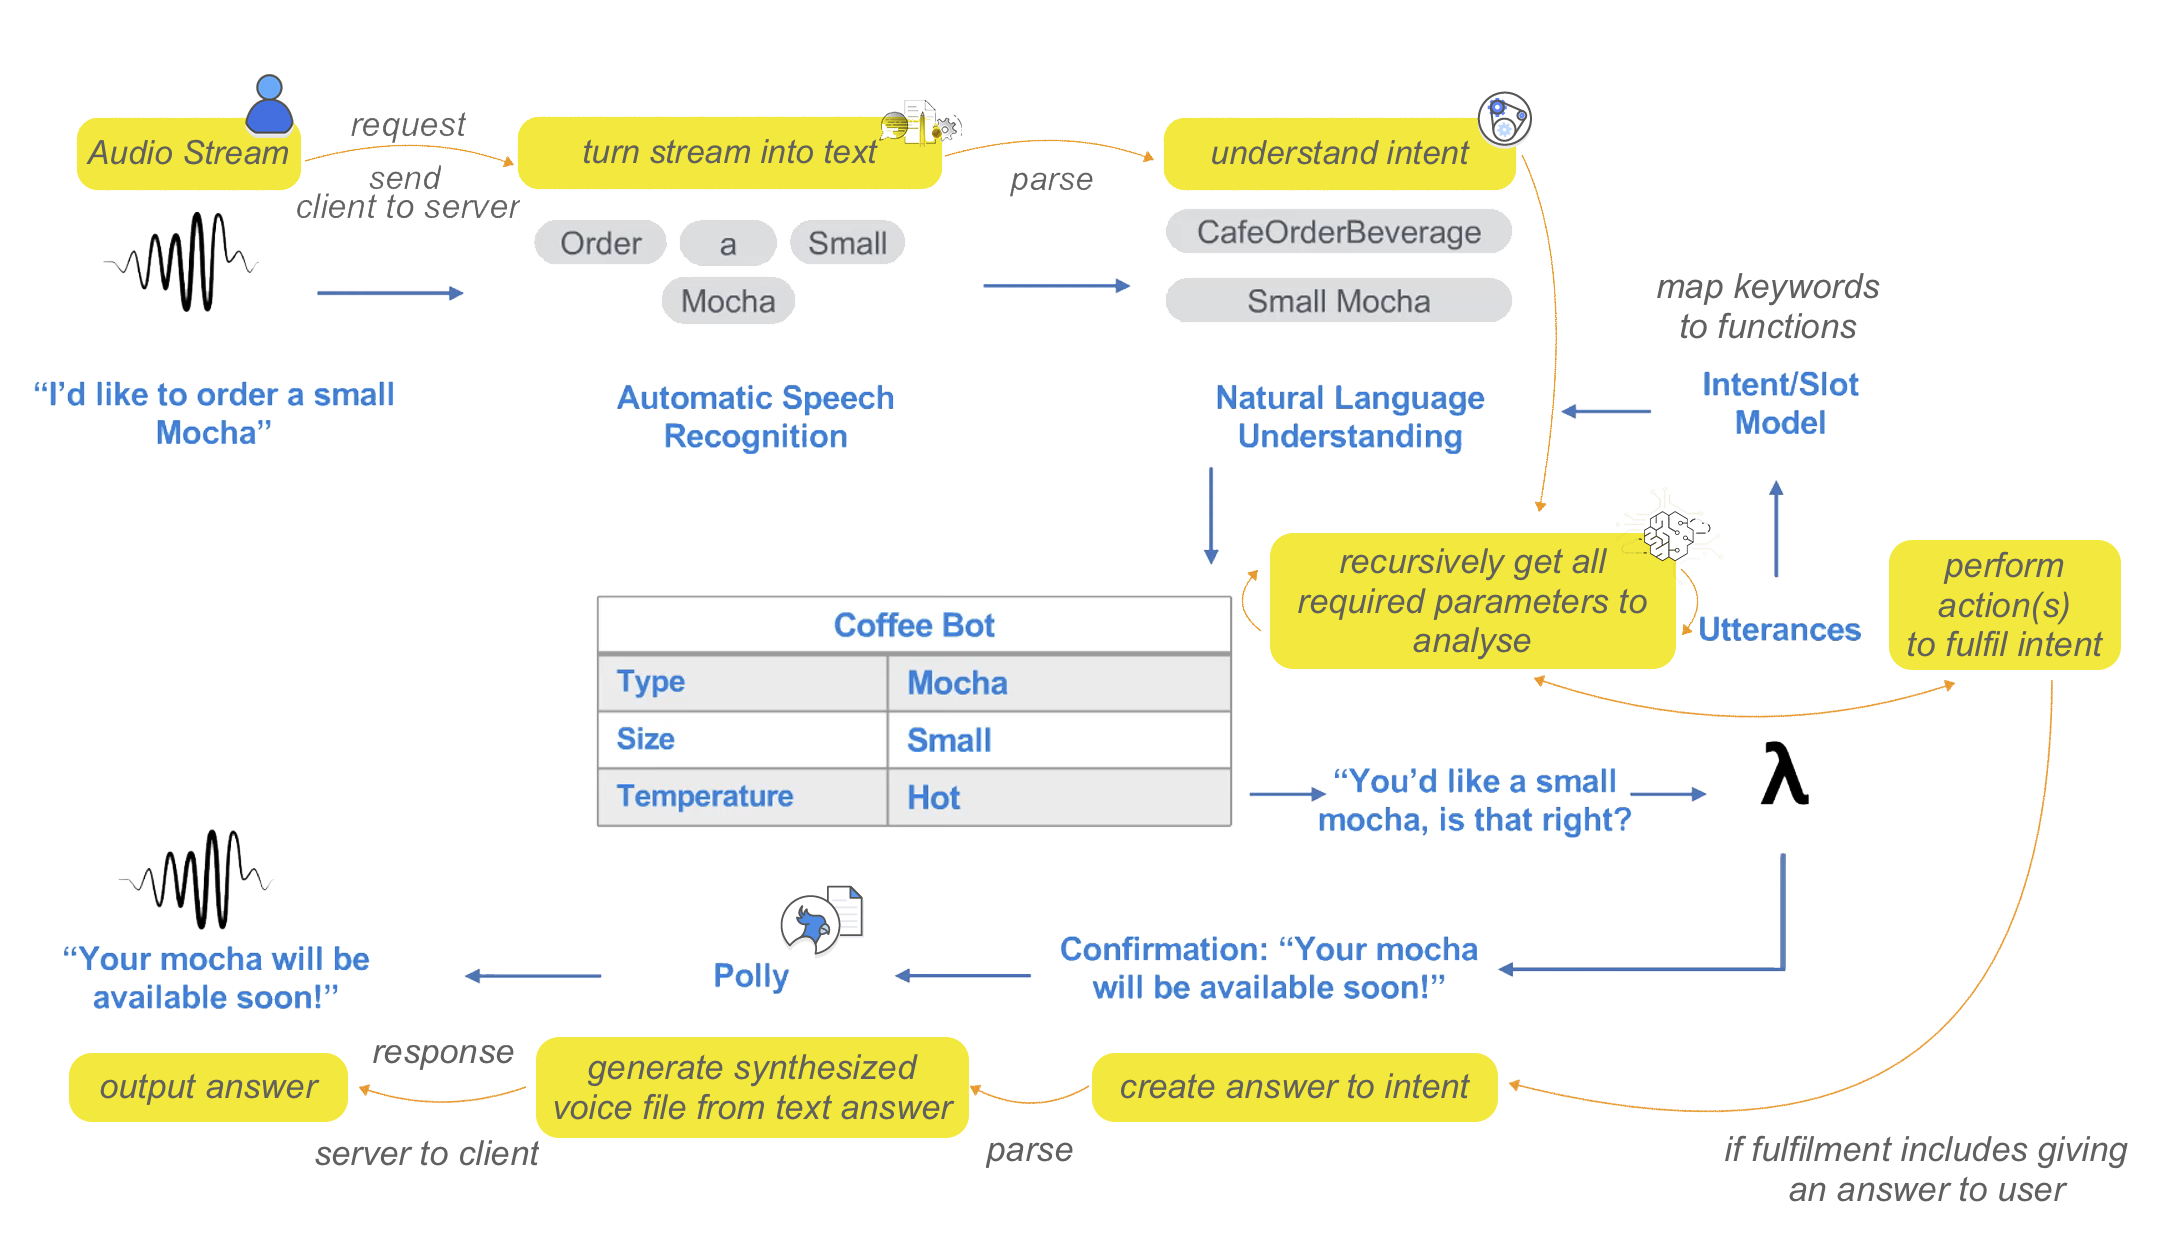
\includegraphics[width=10.5cm]{workflows/awstools.png}
%\end{wrapfigure}

putting different combinations of these and other building blocks interactively together generates the model for Alexa. In a world increasingly operated by Internet of Things (IoT), we describe a possible interaction in the example below for a use case of a hypothetical chatbot that operates a coffee machine using some of these service modules (Figure \ref{lex_interactionExample}).  Although this graphic describes how an end user would combine these modules to set up their own chatbot, this is the same workflow that Alexa uses. Hence, with Amazon's use of its own micro-services we infer that takes advantage of these to build a whole new ecosystem putting Alexa Skill developers as producers, end-users as consumers, and the Amazon website and Alexa App as a marketplace to mediate between the products (Skills) the developers produce to their target customers (end-users, country-specific or worldwide). From a marketing perspective Amazon achieves through Alexa a vertical diversification of its product programme (where existing AWS services result in a new product expanding the value chain) while simultaneously offering an extention of its aggregator-model marketplace model by playing as a mediator between the developers' role and that of end-users % (who of course could be developers, too)
% this is from what I concluded from MKT and GepIT lectures.. Prof. Küpper, Axel / Prof. Klasse-Talke, Kathrin




we can therefore describe the meta-model for Alexa similar as one %to that
of an application with several front-end and back-end components. Unlike in most GUI-based scenarios with an MVC design pattern \cite{wiki:mvc}, where the user uses the \lstinline|controller| to manipulate the \lstinline|model|, which in turn updates the \lstinline|view| appearing to the user, in a VUI scenario, we need to consider that the user's paradigm to the \lstinline|view| component is quite different. Before we dive into the VUI paradigm, we introduce Alexa's own implementation of it for third-party applications. These are broken down into the following elements for users and developers to comprise a holistic ecosystem:




\begin{itemize}
	\item Alexa Skills Kit: although it is hard to define it as a complete SDK for Alexa, it is responsible for compiling the loosely coupled tools provided by AWS and others to act as an interface for the skill from a developer point of view. This fits into the rest of Amazon's scheme of focusing on interoperable micro-services that fit multiple purposes.
	
	%Explain what the ASK SDK does
	
	\begin{itemize}
		\item Alexa Developer Console
		\item ASK Command-Line Interface 
		\item Amazon Voice Interface
	\end{itemize}
	\item Alexa Skills Store for users: where a user can preview the skills before they install it, know if they want it or not and by installing them, the own instance of alexa becomes "smarter" um einen weiteren skill \footnote{das mündet into something where AI becomes smarter then maybe in 5 years the concept of alexa skills won't exist anymore and would be integrated into Alexa's own brain without the user knowing and it would just be a hit or miss kind of thing.} for now the user does not need to think about updates since these happen in the backend. approval makes amazon decide wether versions are good and make the skill better or worse or change things to worse partly
\end{itemize}
Alexa Skills Kit  




\subsection{Amazon Voice Service}
just like other common chat bot constructs, Alexa Skills Kit (ASK) divides the building model into intents~\ref{intents}, utterances and slots. The Fulfilment part is taken care of through Amazon Lambda contains the programming \inote{and business} logic to the interface
\begin{itemize}
	\item Intents
	\
\end{itemize}


\subsection*{Alexa Interfaces}

\begin{table}[htbp]
	\caption{Alexa Devices in Comparision}\label{alexaDeviceTable}
	\centering
	\begin{tabularx}{\textwidth}{ r | l l l l }
		
				& Echo Dot/Echo/Echo Plus/Tap & Echo Spot     & Echo Show     & FireTV \\ \hline
		screen  & n                           & 2.5'' round 		  & 7.0'' 		  & via HDMI Display       \\
%				&							  & (round)		  &				  &				\\
		line out& y      					  & y             & via Bluetooth & via HDMI      \\
	\end{tabularx}
\end{table}

%then comes el software 

hardware \inote{just make a comparison table, which one has a screen, which one has which capabilities with alexa}
Echo, Echo Dot, Tap, FireTV

software
Alexa app is not an alexa interface

while these are possibilities for testing, too,  they are primarily developed with testing in mind
\begin{itemize}
	\item[EchoSim.io]
	\item[Alexa Simulator]
	\item[Reverb]
\end{itemize}



%%%%%%%%%%%%%%%%%%%%%%%%%%%%%%%%%%%%%%%%%%%%%%%%%%%%%%%%%%%%%%%%%%%%%%%%%%%%%





\todo{move / remove what is irrelevant
	In this section, we conduct a short survey of problems we can face with natural language
\subsection*{topology of bots}
\textbf{by platform:}
-API.ai / 
Facebook Messenger Chatbots /	
-wit.ai /
-motion.ai / Flask
\textbf{by category}\\
- leisure /
- \href{https://www.forbes.com/sites/tomaslaurinavicius/2017/04/24/facebook-messenger-bots/\#4f61c16a66d8}{fun bots}  / 
- productivity / 
- more (graph from voicelabs report) \\
- what are classic use cases for their use with prominent examples?\\ Booking tickets (e.g. airline bot)\\ %KLM
- quick survey of respective 'AppStores'\\
\textbf{by purpose}\\
-physical locations (home, office, car, phone, in a business)\\
Information bots\\
\textcolor{magenta}{
	- mention available service types (information system as a "webpage/database")\\
	- vs an interactive bot that gives you customized information on demand
	hier soll der D115 Anwendungsfall "Beauskunftung" kurz erl\"autert werden\\
}
social bots\\
\textcolor{magenta}{
	- with advantages / disadvantages\\
	- fake news / online reviews\\
}
more on AI in bots (optional)\\
\textcolor{magenta}{
	- use of ML\\
	Handyversicherungsbeispiel\\
	- from business perspective, the bot is aiming to sell more polices,\\ 
	- the bot tries to determine if there is a nuance in the user's answer (machine acting as a judge!)
	- e.g. ``how did the phone fall off``
	- MKTG - Aufwand
}


\textbf{eingehen auf}\\
- Wienbot\\
- Singapore / LA / Ask Georgia...\\

}

%#############################################################################
%###################### Related work  ########################################
%#############################################################################

%DELETEME: Related work respresents results from work that handled the same or a similar problem that you are addressing. This work might have used a different approach or might not have been that successful. Finding a paper / work that solved your problem in the same way you were planning to do is not good and you should contact your supervizor for solving this issue. Again, each paper / work has to be connected to your approach: other papers might have not chosen an optimal solution; they might not have been taking care of essential aspects; they might have chosen a different approach and you believe, yours will work better ...

\section{Related Work}
wienbot, singapore etc, d115
\todo{

}

While we have no access to AskGeorgia



%IFTTT Applets for voice commands


\todo{ 2 \P \\
	
	\textbf{- Chatbot vs. human: }
	%what we used to do with facets vs a search mask predicting possible facets - we are at a stage where bots are like altavista..u tell alexa to open a skill like u tell altavista to look in pics or go to lexisnexis to do reserach. we are yet to reach the state of watson like google is to searches
	Analyze differences between bot and human response\\
	%human says long sentences and there is a fluid transition between dialog and monologue 
	-disadvantage: a bot wants a sentence broken down in small pieces to avoid errors in lengthy interpretation\\
	% otherwise, error margin too large.\\
	% this has to do with human language complexity.\\
	- \textbf{Why can't robots understand us:} language ambiguities - the need to understand context\\
	--Syntactical: Homonyme\\ %fly, fly,  presently I’ll present you a present - now, give, gift
	--Semantic:  Methaphors, %“it’s raining cats and dogs”
	sarcasm, %“oh yea, sounds very exciting”
	and puns\\
	--dialects: enunciations\\
	--underlying grammar\\ %“what makes you abcd just now, ELIZA
	--underlying sentiment\\
	-\textbf{NLP Progress:} How does it help in enriching the bot experience\\
	--neural networks: help understanding language patterns and get better over time\\
	--thought vectors: helps connect different words with related meaingns\\
	- \textbf{wrap-up:} can bots replace serivces offered by humans?
	-- mention transition from facets (Altavista) to metasearches to all-in-one (Google). \\
	-- chatbots as enablers in customer service industry\\
	-- conclusion: Although not impossible, it is a bit too far-fetched at this stage.\\
}


%%%%%%%%%%%%%%%%%%%%%%%%%%%%%%%%%%%%%%%%%%%%%


These include lex for.... so-called `Skills' It comes with


\begin{wrapfigure}{r}{1.5cm}
	\caption{text}\label{key}
	
\includegraphics[width=2.5cm]{template/aot_logo}
\end{wrapfigure}

%\item \href{URL}{Amazon Voice Services}
%
%\item 



Intent fulfilment \label{intent_fulfilment}

 
\todo{	
	-  Alexa Skills Kit+ Amazon Voice Services\\
	- mention how ability to react to everything is centralized at alexa somewhere \textbf{talk about SKILLS}\\
	- ability to retain sessions (explain requests/responses - GET/POST)\\
	- fullfilling intents\\
	- nested handlers\\
		\\
		skill service: code - business logic - handles json requests
		skil interface: configuration (developer portal)
		\\
	- difference to Lex \& Polly\\
	\href{https://stackoverflow.com/questions/42982159/differences-between-using-lex-and-alexa}{diff alexa lex}
		
	- Major prob: lex is not in german
- \href{https://www.youtube.com/watch?v=QxgdPI1B7rg}{Alexa Documentation}
}



%%%%%%%




%###################################################################################
%###################### Topic B             ########################################
%###################################################################################
\section{Frameworks and Data Structures}\label{frameworks_structs}


\textcolor{magenta}{-AL: Ich w\"urde erst etwas die Algorithmen und Datenstrukturen (Textanalyse, JSON, ggf. Graphen beschreiben. 
	-AL: Anschlie{\ss}end die Frameworks vorstellen\\ 
	-AL: Wichtig ist: Aus den Beschreibungen eine Schlussfolgerung ableiten, welche Art von L\"osung entwickelt werden soll.\\
for current bot: \\
- Lucene \textbf{as the golden standard}: spell check, unscharfe suche, Tika / detect language / ... \\
- Solr
- explain what's an intent, whats a slot
\url{https://service.berlin.de/virtueller-assistent/virtueller-assistent-606279.php}
\url{https://www.itdz-berlin.de/}
}




\subsection*{Node.js}

AWS Lambda supports multiple runtime environments including Python, Java, C\# and Go. We decide to use Node.js due to its event-driven nature and to take advantage of its non-blocking I/O model. Being single-threaded, Node.js guarantees high performance at large scale with large volumes of requests considered. With its JavaScript (ECMAScript) foundation, no wonder it is becoming a standard in web-apps. Hence, the decision also comes due to the richness of develpers' experience with the implementation for Alexa Skills.
\todo{
	- Server-side, browser side (Chrome V8), App layer, data layer\\
	- because it can read our JSON easily and fast
	- talk about Methodenaufbau (syntax) and firing events
}


\subsection*{Solr}
w lucene w tika w nutch wel habal da if required





%###################################################################################
%###################### Use Case in detail  ########################################
%###################################################################################
\section{The Analysed Scenario as a Use Case}
\subsection*{D115}
\textcolor{magenta}{
	- summarize infobroschuere\_ BMI08324\_screen\_barrierefrei.pdf\\
	-Use case im Detail\\
	-Welche Daten gibt es?\\	  
	-Was sind die Erwartungen?\\ 	
	- wie kann man die G\"ute des Systems beurteilen?\\   
	- Meist sollte man in diesem Kapitel die L\"osung schon im Auge haben, um die Erwartungen so zu formulieren, dass die L\"osung auch geeignet ist?\\ 
}




\subsection*{currently deployed bot}



\textcolor{magenta}{
	- dienstleistungen.json structure (finding the info through hierarchical nodes)\\
	- interpreting the nodes as intents
	- traversing the nodes (one level up then to next node)
	- no session/no persistence
	%x	x	x
	%ooo ooo ooo
	%try first, go to second (kosten, zeit, rechtsgrundlage, ..) skip one if it has already been suggested.. hinweis..that is built into the xml
	%
	%the live service is different than the one at DAI
}

%%%%%%%%%%%%%%%%%%%%%

OnLaunch
IntentHandler
intent is triggered by utterence
account verlinkungen etc

%\Tree [.Dienstleistungen.json created [.VP [.V is ] NP ] ]
%
%\Tree[.Dienstleistungen.json 	
%	[.NP [.Det \textit{the} ]
%		[.N\1 [.N \textit{package} ]]]
%	[.I\1 [.I \textsc{3sg.Pres} ]
%		[.VP [.V\1 [.V \textit{is} ]
%			 	   [.AP [.Deg \textit{really} ]
%				  		[.A\1 [.A \textit{simple} ]
%							  \qroof{\textit{to use}}.CP ]]]]]]]

provided in JSON for value lookup, there are


explain how the json nodes map to intents and cores in solr etc


\begin{figure}[h!]
	\caption{\lstinline|Dienstleistungen.json|  - Primary Nodes}
	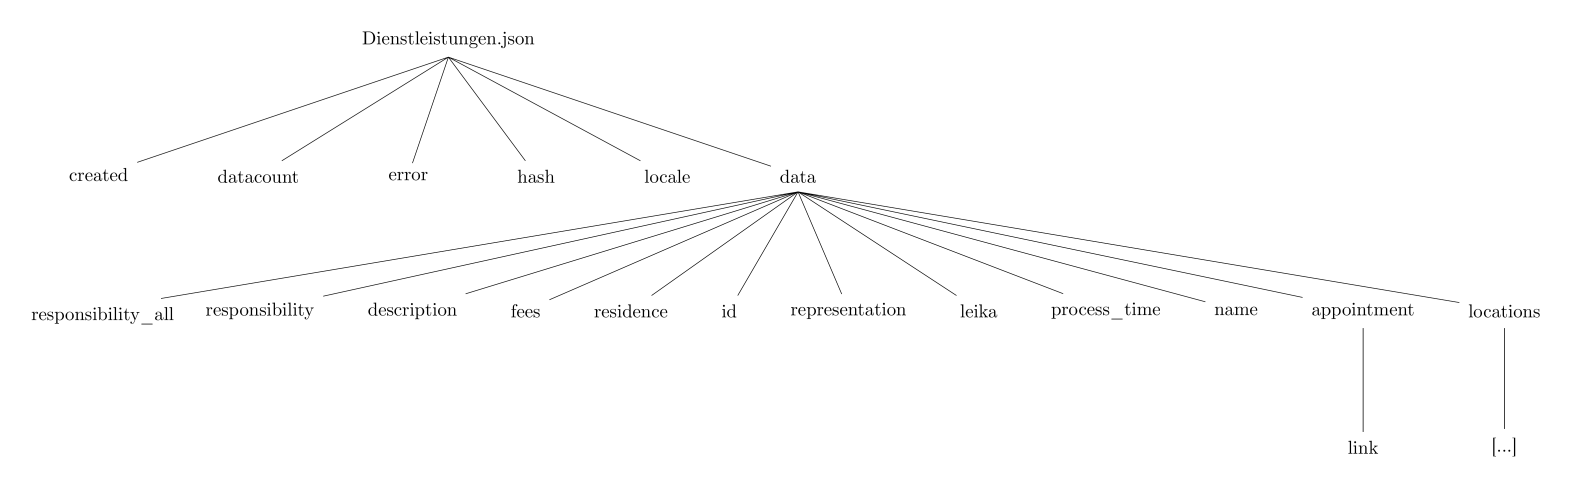
\includegraphics[width=\textwidth]{DLprim}
\end{figure}

\begin{figure}[h]
	\caption{\lstinline|Dienstleistungen.json| - secondary Nodes}
	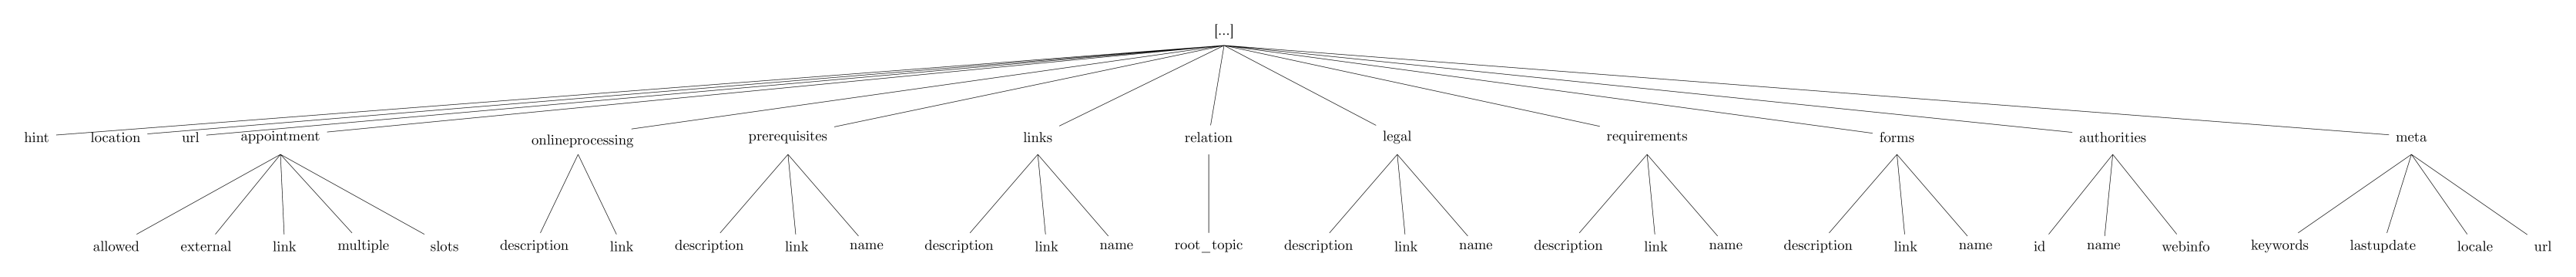
\includegraphics[width=\textwidth]{DLsec}
\end{figure}

\begin{itemize}
	\item 616 Intents as \lstinline|data|, each containing
	\todo{missing variables e.g. are required papers, flag: persönliche Vorsprache ja nein, ...}
	\begin{itemize}
		\item \lstinline|<string> responsibility| denoting in which city halls a service is available
		\item \lstinline|<boolean> responsibility_all| a flag set to true in case the service is available in all local authority offices / service points
		\item \lstinline|<HTML list string> description| not unified and includes text
		\item  \lstinline|<string> not unified and might need to have an \lstinline|int| added to it and set to 0 in case service is free
		\item \lstinline|<int>residence|
		\item \lstinline|<int>id|
		\item \lstinline|representation|
		\item \lstinline|<long>leika|
		\item \lstinline|<string> process_time| need to derive minimum, average and maximum service times instead of a string, as well as conditions 
		\item \lstinline|<string> name| the name of the service that would make sense to a human
		\item \lstinline|<node> appointment| with 
		\begin{itemize}
			\item \lstinline|link| (Key value with URL to /terminveinbarung page) - check if orphan or if it is for each beh\"orde and in that case how it gets the right one
		\end{itemize}	 
		\item \lstinline|<node> locations| 
		\begin{itemize}
			\item \lstinline|hint|
			\item \lstinline|<int> location| one of the 12 authorities
			\item \lstinline|url| of that service at that authority
			\item \lstinline|<node> appointment| (a second one)
			\begin{itemize}
				\item 
			\end{itemize}
		\end{itemize}
		
		\item \lstinline|<node> onlineprocessing|
		\item \lstinline|<node> prerequisites|
		\item \lstinline|<node> links|
		\item \lstinline|<node> relation|
		\item \lstinline|<node> legal|
		\item \lstinline|<node> requirements|
		\item \lstinline|<node> forms|
		\item \lstinline|<node> authorities|
		\item \lstinline|<node> meta|										
	\end{itemize}
\end{itemize}



%###################################################################################
%###################### Topic C             ########################################
%###################################################################################
\section{Implementation Possibilities}

\textcolor{magenta}{
- structure of Hitlist on berlin.de  is provided by ITDZ -  as opposed to Versicherungsfirma z.B (ML tries to detect irregular patterns in case customer is lying).
- unfortunately forums vs. FAQs did not work. if i want assistance, i want the customer to tell me the model number - and forums have mostly Schrott!\\
what the bot curently achieved is at least not give wrong answers, sometimes says idk but it doesnt confuse u. same attitude like in german shops (nur unpassende antworten sind frustrierend!\\
\\
-Vorgehensweise: XML -> index \"uber Lucene - >solr knoten...based on sth like when i say \" am 10. august\" it gets me masalan events..aha august ist ein monat, monat relates to calendar, calendar relates to events
}